\chapter{Discussion}\label{ch:Discussion}

% + a lot of boost for solar
% + Linear, good for control
% + 2 switches reducte ripple in source and load
% + single switch can still run 
% - more components
% - voltage drops
% ? efficiency

The first advantage of the converter is the high conversion ratio that is very interesting for applications as PV arrays. As the results from simulation had shown before that the high conversion ratios are possible conversion ratios of over 22 have been reached in testing of the hardware.


The other big advantage of this converter is the linear dependency of the duty cycle to the voltage output. The task for controllers for solar panels is to extract the maximum energy which is a difficult task on its own. 
By using a linear converter the controller can track this optimal point easier as the additional non-linearity is not added to the system.


With a PWM pattern with minimum overlap applied to the MOSFETs the two inductors charge after each other, reducing the current ripple on the input. This equalling of the load is very good for the solar panels as its lifetime can be shorted by ripple. \cite{Joseph_isbn978-3-8007-3343-9} % https://publik.tuwien.ac.at/files/PubDat_210330.pdf
%\todo[color=c07,inline]{Ref}
Another option is to run both MOSFETs on the same PWM signal.
Then the voltage ripple of the top and bottom half of the circuit will cancel each other out, reducing the ripple on the load. 

Another advantage of heaving two converters combined in one, is that one half can have a fault and the second half still works.
If it would be implemented in the controller the converter set up in a remote PV array would continue operating after detecting that components have failed. 
The conversion ratio would be limited to half of the original but on high sun intensity it would be still functional until the converter is getting replaced.


Disadvantage of the converter is that it needs more components, increasing the cost and the risk of failure.
Also the Cockroft-Walton Multiplier is using a lot of diodes that cause big voltage drops on the output.

In hardware testing the results where far off of the theoretical values.
The main reason for that is the selection of the components: 
The inductor is limited to currents of 3A, limiting the input while the oversized diodes where made for higher currents and are not operating efficiently with the low currents we tested with.
Also the capacitor C1 had high thermal losses in testing.

When comparing the measurements of this topology and a CBC with the same components (L=135$\mu$H, C=2.2$\mu$F, R=2k$\Omega$, same MOSFET, same diode)
and looking at the efficiency the results are very different.
A graph of measured efficiencies with interpolation can be seen in Figure \ref{fig:Efficiencycomparison}.
While on the CBC loses a lot of its efficiency after duty cycles of 70\% the multi stage 2NX Interleaved Boost Converter reached even higher efficiency on higher duty cycles in the tests.

\begin{figure}[H]
	\begin{center}
   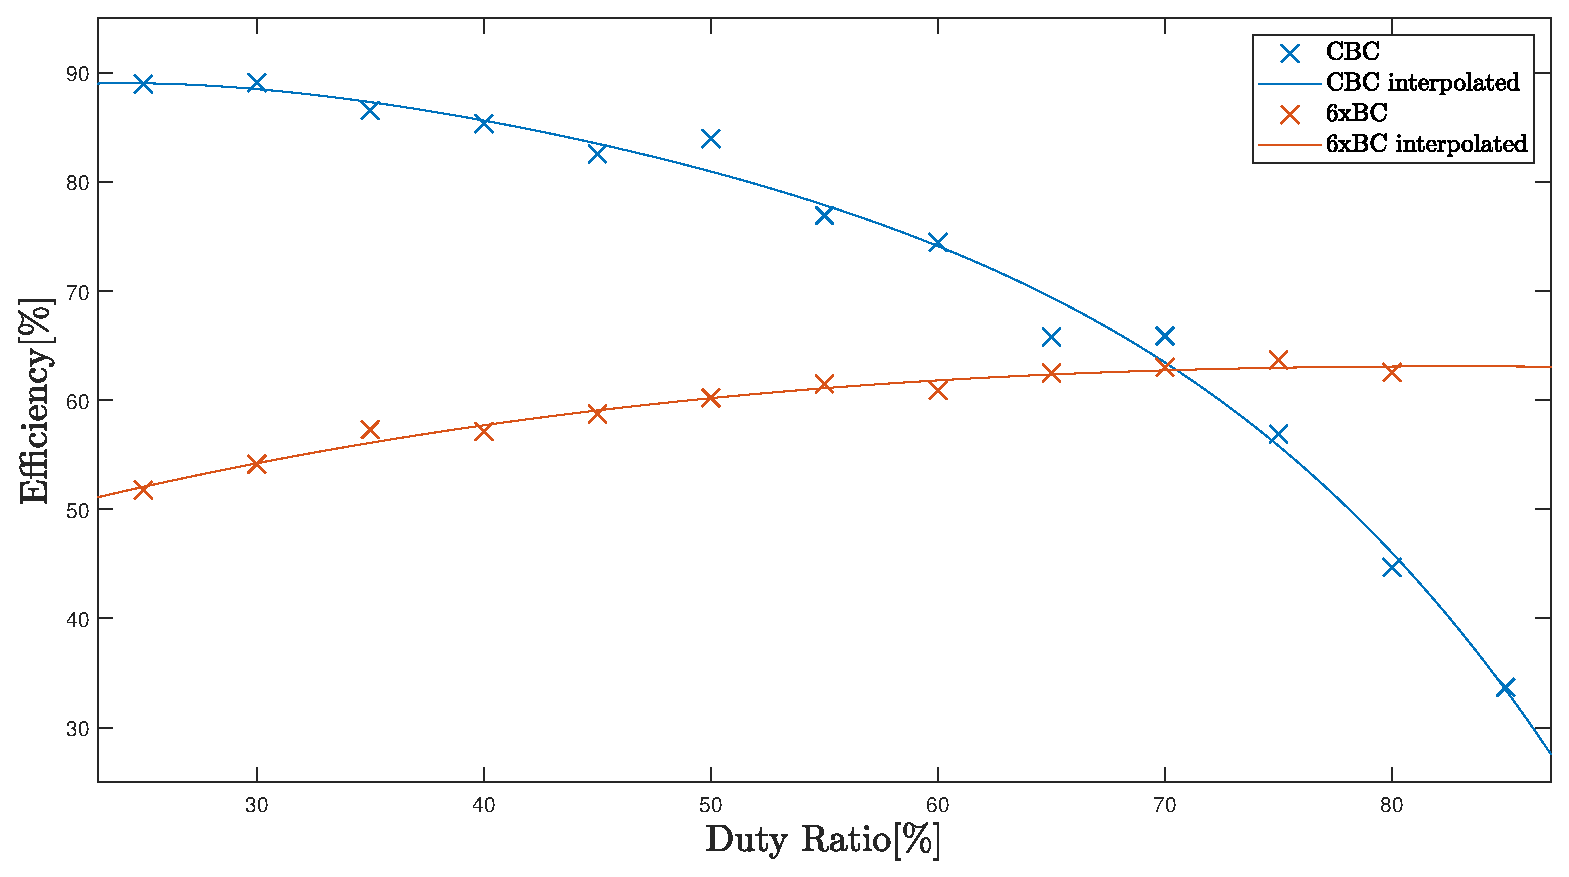
\includegraphics[width=0.8\textwidth]{figures/Efficiencycomparison.eps}
	\end{center}
	\vspace{-4mm}
	\caption{Comparison of efficiency with a conventional BC}
	\label{fig:Efficiencycomparison}
\end{figure}